\documentclass[DM,toc]{lsstdoc}
\usepackage{booktabs}

\title[Qserv Test Fall 2016]{Qserv Fall 16 Large Scale Tests/KPMs}
\author{Vaikunth~Thukral}
\date{2017-05-09}
\setDocRef{DMTR-16}

\setDocAbstract{%
This document contains results of the large scale tests at 20\% DR1 capacity
that were run on CC-IN2P3 cluster during February-March 2017.

For comparisons, the previous large scale test can be found in \citeds{DMTR-13}.
}

\begin{document}
\maketitle

\section{Dataset Information}\label{dataset-information}

\begin{longtable}[]{@{}llll@{}}
\toprule
\textbf{Table} & \textbf{Row Count} & \textbf{.MYD size {[}TB{]}} &
\textbf{.MYI size {[}TB{]}}\tabularnewline
\midrule
\endhead
Object & 3,777,968,880 & ~4.6 & 0.1\tabularnewline
Source & 69,744,689,072 & 33.6 & 3.6\tabularnewline
ForcedSource & 344,034,271,380 & 11.0 & 8.7\tabularnewline
\bottomrule
\end{longtable}

Total MySQL data dir size: 62.4 TB

DR1 numbers are available at~
\href{https://www.lsst.org/scientists/keynumbers}{LSST Key
Numbers}~under "Data Releases"

Object and Source are now at \textasciitilde{}20\% of DR1 level and
ForcedSource has more than 20\% of DR1.

\section{Hardware}\label{hardware}

\begin{itemize}
\item
  50 nodes:

  \begin{itemize}
  \item
    DELL PowerEdge R620
    (\href{http://www.dell.com/downloads/global/products/pedge/en/Dell_PowerEdge_R620_Spec_Sheet.pdf}{Dell
    Spec Sheet}) for nodes 1-25
  \item
    DELL PowerEdge R630
    (\href{http://i.dell.com/sites/doccontent/shared-content/data-sheets/en/Documents/Dell-PowerEdge-R630-Spec-Sheet.pdf}{Dell
    Spec Sheet}) for nodes 26-50
  \end{itemize}
\item
  2 x Processors Intel Xeon E5-2603v2 @ 1.80 Ghz 4 core
\item
  10 MB cache, 6.4 GT/s, 80W
\item
  Memory 16 GB DDR-3 @ 1600MHz (2x8GB)
\item
  2 x hard drive 250GB SATA 7200 Rpm 2,5" - hotplug =\textgreater{} OS
\item
  8 x hard drive 1 TB Nearline SAS 6 Gbps 7200 Rpm 2,5"
\item
  hotplug =\textgreater{} DATA
\item
  1 x card RAID H710p with 1 GB nvram
\item
  1 x card1 GbE 4 ports Broadcom® 5720 Base-T
\item
  1 x card iDRAC 7 Enterprise
\end{itemize}

\section{Testing methodology and
summary}\label{testing-methodology-and-summary}

The cluster is divided into two sets of 25 nodes each, and each
sub-cluster has the 20\% DR1 dataset loaded in. These KPM tests were
performed on the second half, on nodes ccqserv125-ccqserv149~(DR1 is
expected to be on~92 nodes)

Queries are selected from a query pool that is divided into "types"
representing different usage patterns as well as expected support for
baseline requirements. Threads in the count of number of simultaneous
queries to be tested are spawned, each managing an open connection to
the qserv proxy and repeatedly picking random queries for its designated
pool while sleeping when required.

The actual program that we used to drive the testing can be found
at:~\href{https://github.com/lsst/qserv/blob/master/admin/tools/docker/deployment/in2p3/runQueries.py}{runQueries.py}

\subsection{\texorpdfstring{\textbf{Short
queries}}{Short queries}}\label{short-queries}

\begin{itemize}
\item
  Single object selection by ID: 0.18 sec

  \begin{itemize}
  \item
    SELECT * FROM Object WHERE deepSourceId = 16968353272299750
  \end{itemize}
\item
  Small spatial area selection from Object: 0.52 sec

  \begin{itemize}
  \item
    SELECT COUNT(*) FROM Object WHERE qserv\_areaspec\_box(42.247928,
    38.874077, 42.273855, 39.034748)
  \end{itemize}
\end{itemize}

\subsection{\texorpdfstring{\textbf{Full table scans, single query at
a
time}}{Full table scans, single query at a time}}\label{full-table-scans-single-query-at-a-time}

\begin{itemize}
\item
  Object: \textasciitilde{}7 min

  \begin{itemize}
  \item
    SELECT ra, decl, u\_psfFlux, g\_psfFlux, r\_psfFlux FROM Object
    WHERE y\_shapeIxx BETWEEN 20 AND 20.2
  \end{itemize}
\item
  Source: \textasciitilde{}41 min

  \begin{itemize}
  \item
    SELECT COUNT(*) FROM Source WHERE flux\_sinc BETWEEN 1 AND 1.1
  \end{itemize}
\item
  ForcedSource: \textasciitilde{}26 min

  \begin{itemize}
  \item
    SELECT COUNT(*) FROM ForcedSource WHERE psfFlux BETWEEN 0.1 AND 0.2
  \end{itemize}
\end{itemize}

\subsection{\texorpdfstring{\textbf{Full table joins, single query at
a
time}}{Full table joins, single query at a time}}\label{full-table-joins-single-query-at-a-time}

\begin{itemize}
\item
  Object x Source: \textasciitilde{}56 min (See the "Notes and
  Observations" section for details)

  \begin{itemize}
  \item
    SELECT o.deepSourceId, s.objectId, s.id, o.ra, o.decl FROM Object o,
    Source s WHERE o.deepSourceId=s.objectId AND s.flux\_sinc BETWEEN
    0.3 AND 0.31
  \end{itemize}
\item
  Object x ForcedSource: \textasciitilde{}38 min

  \begin{itemize}
  \item
    SELECT o.deepSourceId, f.psfFlux FROM Object o, ForcedSource f WHERE
    o.deepSourceId=f.deepSourceId AND f.psfFlux BETWEEN 0.13 AND 0.14
  \end{itemize}
\end{itemize}

\subsection{\texorpdfstring{\textbf{Concurrent scans and stress
test}}{Concurrent scans and stress test}}\label{concurrent-scans-and-stress-test}

\begin{itemize}
\item
  2 Object scans: \textasciitilde{}8 min
\item
  5 Object scans: \textasciitilde{}8 min~(this shows that shared scans
  implemented in W16 work as intended)
\item
  Able to run up to 35 (30 on Object, 3 on Source and 2 on ForcedSource)
  scans together~--- Object scans \textless{} 1h and Source scans
  \textless{} 1.5h
\item
  Attempt to run 50 scans causes the proxy to fail, solution is targeted
  in multi-czar deployment in the future
\end{itemize}

\subsection{\texorpdfstring{\textbf{\emph{Typical load test 60 LV +
10 HV (+10\% if
possible)}}}{Typical load test 60 LV + 10 HV (+10\% if possible)}}\label{typical-load-test-60-lv-10-hv-10-if-possible}

\begin{itemize}
\item
  60 low volume and 10 high volume queries (4 scans for Object, 1 scan
  for Source, 1 scan for ForcedSource, 2 Object-Source joins, 1
  Object-ForcedSource join and 1 NearNeighbor query), all running
  simultaneously with appropriate sleep in between queries to enforce
  the mix we are aiming for. We also introduce a new metric to quantify
  system performance, \textbf{Q}uery \textbf{T}hrough\textbf{P}ut, or
  \textbf{QTP}
\item
  During 24 hours we completed:

  \begin{itemize}
  \item
    571,029 Low Volume queries finished --- Baseline:
    \textasciitilde{}10 sec per query, 432,000 queries in 24h

    \begin{itemize}
    \item
      Achieved Low Volume QTP: \textbf{396 queries/minute}
    \end{itemize}
  \item
    108 Object scans --- Baseline: \textasciitilde{}1h per query, or 96
    in 24h
  \item
    2 Source scans ---~Baseline: \textasciitilde{}12h per query, or 2 in
    24h
  \item
    2 ForcedSource scans~--- Baseline: \textasciitilde{}12h per query,
    or 2 in 24h
  \item
    4 Object-Source joins ---~~Baseline: \textasciitilde{}12h per query
    or 4 in 24h
  \item
    2 Object-ForcedSource joins~--- Baseline: \textasciitilde{}12h per
    query or 2 in 24h
  \item
    27 NearNeighbor queries~--- Baseline: \textasciitilde{}1h per query,
    or 24 in 24h

    \begin{itemize}
    \item
      Achieved High Volume QTP: \textbf{6 queries/hour}
    \end{itemize}
  \end{itemize}
\item
  Average output:

  \begin{itemize}
  \item
    Overall size of Low Volume results was \textasciitilde{}70GB:
    \textbf{128 KB/query}
  \item
    Overall size of High Volume results was \textasciitilde{}7GB:
    \textbf{48 MB/query}
  \end{itemize}
\item
  Average times:

  \begin{itemize}
  \item
    Low Volume queries~\textbf{3.23 sec/query} --- Baseline: should be
    under 10
    sec\\[2\baselineskip]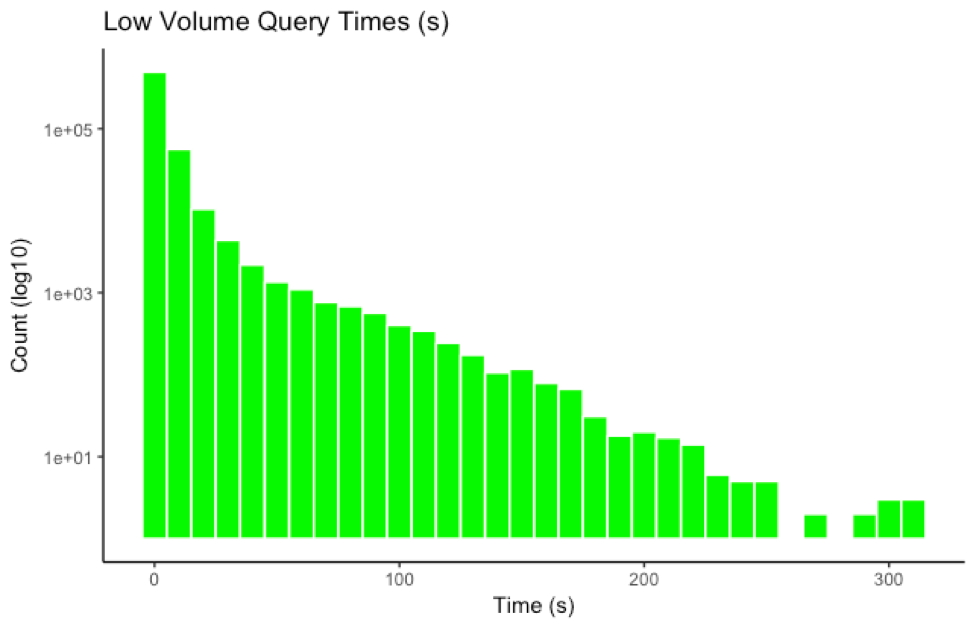
\includegraphics[width=6.50764in,height=4.18472in]{Picture1}

    \begin{itemize}
    \item
      Histogram for all Low Volume query times, note the log scale on
      the Y axis
    \end{itemize}
  \item
    Object scans \textbf{15.15 min/query} ~--- Baseline: should be under
    1 hour
  \item
    Source scans \textbf{2.7 hr/query} --- Baseline: should be under 12
    hours
  \item
    ForcedSource scans~\textbf{2.7 hr/query}~--- Baseline: should be
    under 12 hours
  \item
    Object-Source joins~\textbf{2.7 hr/query} ---~Baseline: should be
    under 12 hours
  \item
    Object-ForcedSource joins~\textbf{2.7 hr/query}~---~Baseline: should
    be under 12 hours
  \item
    NearNeighbor queries~\textbf{16.6 min/query}~---~Baseline: should be
    under 12
    hours\\[2\baselineskip]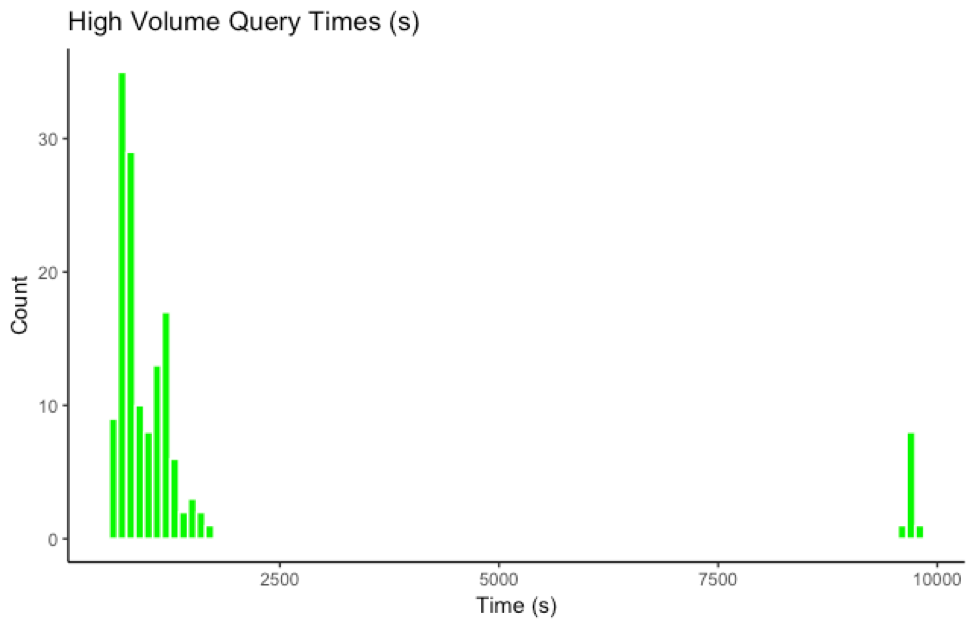
\includegraphics[width=6.50764in,height=4.18472in]{Picture2}

    \begin{itemize}
    \item
      Histogram for all High Volume query times, note the clear
      difference in Object and Source scans
    \end{itemize}
  \end{itemize}
\item
  Observations:

  \begin{itemize}
  \item
    Tests were able to run exactly 10\% faster than the attempted mix
    for Low Volume queries and Object scans (due to the short time frame
    of these queries)
  \item
    Scan scheduling implemented in W16 works with scans on each table
    type running in approximately the same amount of time

    \begin{itemize}
    \item
      For correct scan scheduling and query planning, mysql statistics
      have to be generated. Future work for this is planned
    \item
      Issues were uncovered with returning large result sizes. Future
      testing will take this into account
    \item
      Due to order-of-magnitude increase in output size, average times
      for Low Volume queries has increased due to tests running from one
      submit node
    \item
      For these issues, see~
      \href{https://jira.lsstcorp.org/browse/DM-9757}{DM-9757} - Getting
      issue details... STATUS ~
      \href{https://jira.lsstcorp.org/browse/DM-10360}{DM-10360} -
      Getting issue details... STATUS ~and~
      \href{https://jira.lsstcorp.org/browse/DM-10366}{DM-10366} -
      Getting issue details... STATUS
    \end{itemize}
  \end{itemize}
\end{itemize}

\subsection{\texorpdfstring{\textbf{\emph{Heavy load test 100 LV + 20
HV (+10\% if
possible)}}}{Heavy load test 100 LV + 20 HV (+10\% if possible)}}\label{heavy-load-test-100-lv-20-hv-10-if-possible}

\begin{itemize}
\item
  100 low volume and 20 high volume queries (8 scans for Object, 2 scans
  for Source, 2 scans for ForcedSource, 4 Object-Source joins, 2
  Object-ForcedSource join and 2 NearNeighbor queries), all running
  simultaneously with appropriate sleep in between queries to enforce
  the mix we are aiming for
\item
  During 24 hours we completed:

  \begin{itemize}
  \item
    814,989 Low Volume queries
  \item
    129 Object scans
  \item
    4 Source scans
  \item
    4 ForcedSource scans
  \item
    8 Object-Source joins
  \item
    2 Object-ForcedSource joins
  \item
    54 NearNeighbor queries
  \end{itemize}
\item
  Average Output:

  \begin{itemize}
  \item
    Overall size of Low Volume results was
    \textasciitilde{}130GB:~\textbf{160 KB/query}
  \item
    Overall size of High Volume results was \textasciitilde{}8GB:
    \textbf{38 MB/query}
  \end{itemize}
\item
  Average times:

  \begin{itemize}
  \item
    Low Volume queries~\textbf{9.98 sec/query}
  \item
    Object scans~\textbf{24 min/query}
  \item
    Source scans~\textbf{4.44 hr/query}
  \item
    ForcedSource scans~\textbf{4.44 hr/query}
  \item
    Object-Source joins~\textbf{4.44 hr/query}
  \item
    Object-ForcedSource joins~\textbf{4,44 hr/query}
  \item
    NearNeighbor queries~\textbf{24 min/query}
  \end{itemize}
\item
  Observations:

  \begin{itemize}
  \item
    Did not finish expected number of Object scans
  \item
    Average size of High Volume query results lowered due to fewer
    completed Object scans
  \item
    Low Volume queries still finished under the baseline of 10 seconds
  \end{itemize}
\end{itemize}

\section{Notes and Observations}\label{notes-and-observations}

\begin{itemize}
\item
  \emph{Concurrency maintained:}~With double the data from S15 we
  successfully ran simultaneous queries up to and more than the baseline
  requirements for 20\% DR1
\item
  \emph{Robustness improved:}~Although the tests were run for 24 hours
  in S15 too, these test runs have been performed multiple times and
  continuously over weeks without any Qserv services failing or needing
  restarts
\item
  \emph{Shared Scan implementation:}~Qserv is able to handle
  successively larger number of scans on the same table and perform them
  for a similar cost/time.~
\end{itemize}

\section{Query Templates Used}\label{query-templates-used}

The actual query pool used in these tests is listed
\href{file:////download/attachments/54854103/query_pools.txt\%3fversion=1\&modificationDate=1494281645000\&api=v2}{here}.
A sample of the query types used in each category is listed below.

\begin{itemize}
\item
  Trivial query that retrieves one row, using index
\end{itemize}

SELECT * FROM Object WHERE objectId = \textless{}objId\textgreater{}

\begin{itemize}
\item
  Counts
\end{itemize}

SELECT COUNT( * )~FROM Object

SELECT COUNT( * )~FROM Source

SELECT COUNT( * )~FROM ForcedSource

\begin{itemize}
\item
  Spatially restricted query, small area of sky, should return small
  number of rows (say \textless{}100)
\end{itemize}

SELECT COUNT( * )\\
FROM Object\\
WHERE ra\_PS BETWEEN 1 AND 2\\
AND decl\_PS BETWEEN 3 AND 4\\
\{quote\}

\begin{itemize}
\item
  Full table scan, use some column in WHERE that is not indexes, make
  sure the number of results returned is sane (eg thousands, not
  millions)
\end{itemize}

SELECT objectId, ra\_PS, decl\_PS, \textless{}few other
columns\textgreater{}\\
FROM Object\\
WHERE fluxToAbMag(iFlux\_PS) - fluxToAbMag(zFlux\_PS) \textgreater{} 4

\begin{itemize}
\item
  Aggregation
\end{itemize}

SELECT COUNT(*) AS n,\\
AVG(ra\_PS),\\
AVG(decl\_PS), chunkId\\
FROM Object\\
GROUP BY chunkId

\begin{itemize}
\item
  Near neighbor
\end{itemize}

SELECT COUNT(*)\\
FROM Object o1, Object o2\\
WHERE qserv\_areaspec\_box(-5,-5,5,-5)\\
AND scisql\_angSep(o1.ra\_PS, o1.decl\_PS, o2.ra\_PS, o2.decl\_PS)
\textless{} 0.1

\begin{itemize}
\item
  Joins
\end{itemize}

SELECT o.objectId, s.sourceId, ra\_PS, decl\_PS, \textless{}few other
columns\textgreater{}\\
FROM Object\\
JOIN SOURCE USING (objectId)\\
WHERE fluxToAbMag(iFlux\_PS) - fluxToAbMag(zFlux\_PS) \textgreater{} 4\\
AND \textless{}some restriction from source table\textgreater{}~

\bibliography{lsst}
\end{document}
